\documentclass{beamer}
\usepackage[czech]{babel}
\usepackage[utf8]{inputenc}
\usepackage{fontenc}
\usepackage{graphicx}

\graphicspath{ {img/} }


\usetheme{Boadilla}
\title{Semestrální práce MI-IOT}
\subtitle{Malá meteo statnice}
\author{Tomáš Šimáček}
\institute[ČVUT]{České vysoké učení technické}
\date{\today}

\begin{document}

	\begin{frame}
	\titlepage
	\end{frame}
	
	\begin{frame}
		\frametitle{Záměr}
		\begin{itemize}
			\item Malá meteo statnice
			\item Zaznamenávání teploty
			\item Zaznamenávání vlhkosti vzduchu
			\item V určitých intervalech nebo při zaznamenání pohybu
		\end{itemize}
	\end{frame}

	\begin{frame}
		\frametitle{Senzory}		
		\begin{columns}
			\column{0.5\textwidth}	
				\begin{figure}
					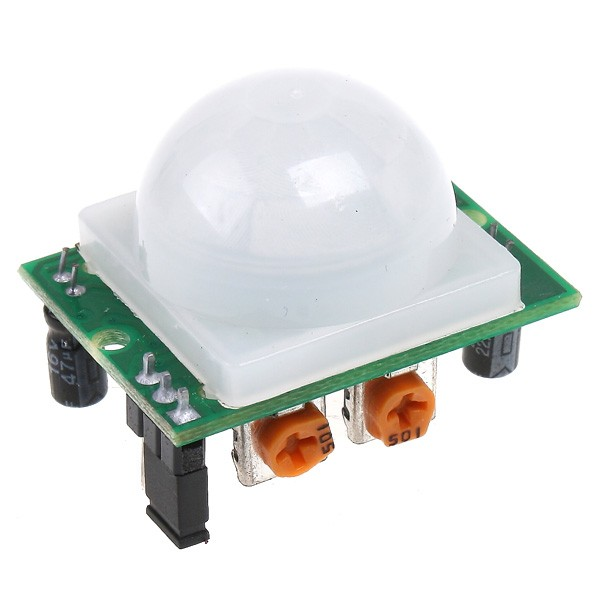
\includegraphics[scale=0.2]{pir.jpg}	
					\caption{PIR čidlo}
				\end{figure}		
				
			\column{0.5\textwidth}				
				\begin{figure}
					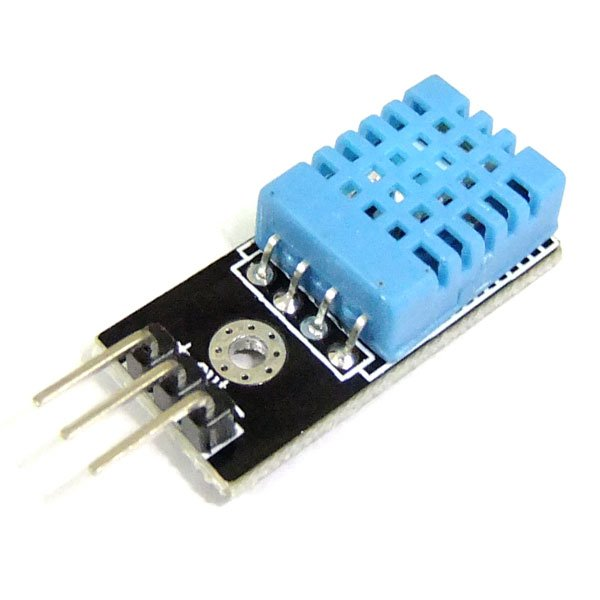
\includegraphics[scale=0.2]{humidity.jpg}			
					\caption{Senzor teploty a vlhkosti}
				\end{figure}		
		\end{columns}				
	\end{frame}

	\begin{frame}
		\frametitle{Rozhraní}
		\begin{itemize}
			\item Webové rozhraní
			\item Přístup přes internet
			\item JSON, graf průběhu teploty a vlhkosti 			
		\end{itemize}
	\end{frame}

\end{document}